\documentclass[11pt,a4paper]{article}

\usepackage[margin=1in]{geometry}
\usepackage[T1]{fontenc}
\usepackage[utf8]{inputenc}
\usepackage{lmodern}
\usepackage{microtype}
\usepackage{graphicx}
\usepackage{booktabs}
\usepackage{longtable}
\usepackage{tabularx}
\usepackage{array}
\usepackage{multirow}
\usepackage{xcolor}
\usepackage{enumitem}
\usepackage{amsmath}
\usepackage{amssymb}
\usepackage{float}
\usepackage{listings}
\usepackage{hyperref}
\usepackage{fancyhdr}

\hypersetup{
  colorlinks=true,
  linkcolor=blue!50!black,
  citecolor=blue!50!black,
  urlcolor=blue!50!black,
  pdftitle={Reliable In-Car Voice Assistance with Target Speaker Extraction},
  pdfauthor={Car-TSE research project}
}

\definecolor{codegray}{gray}{0.95}
\definecolor{darkgreen}{rgb}{0.0,0.35,0.0}
\definecolor{darkred}{rgb}{0.55,0.0,0.0}
\lstset{
  basicstyle=\ttfamily\scriptsize,
  backgroundcolor=\color{codegray},
  frame=single,
  breaklines=true,
  columns=fullflexible,
  keepspaces=true,
  showstringspaces=false
}

\newcolumntype{Y}{>{\raggedright\arraybackslash}X}
\newcommand{\good}{\textcolor{darkgreen}{\textbf{evidence present}}}
\newcommand{\blocked}{\textcolor{darkred}{\textbf{blocked}}}
\newcommand{\proxy}{\textit{proxy only}}
\newcommand{\pathnote}[1]{\texttt{\detokenize{#1}}}
\newcommand{\metric}[1]{\textbf{#1}}

\pagestyle{fancy}
\fancyhf{}
\lhead{Car-TSE research report}
\rhead{2026-10-14}
\cfoot{\thepage}
\setlength{\headheight}{14pt}

\title{\textbf{Reliable In-Car Voice Assistance with Target Speaker Extraction}\\
\large Full system report, benchmark record, ablations, latency, and Jetson transfer package}
\author{Car-TSE research project}
\date{14 October 2026}

\begin{document}
\maketitle

\begin{center}
\fbox{\parbox{0.94\linewidth}{
\textbf{Evidence status.} This is a research-engineering report, not a
production sign-off. The project has zero consented real-driver sessions and
no matching six-input capture device. All positive end-to-end numbers are
synthetic or cross-corpus proxies; the negative streams are useful diagnostic
exposures but are not a substitute for a speaker-consistent vehicle study.
The current readiness label is \texttt{research\_engineering\_preview} and
\texttt{production\_ready=false}.
}}
\end{center}

\tableofcontents
\newpage

\section{Executive summary}

\subsection{Goal}

The project asks whether an in-car assistant can reliably hear a driver,
recognize the wake word "Marvin", understand the command that follows, and
avoid acting on passenger or background speech. The intended operating
conditions include four cabin microphones, vehicle noise, overlapping
passenger speech, optional playback reference audio, short speaker
enrollment, and a constrained edge deployment.

\subsection{System}

The implemented cascade is:

\begin{enumerate}[leftmargin=*]
  \item four-channel cabin audio and an optional aligned playback reference;
  \item a learned cabin front end and a 16 kHz SpEx+-style target-speaker
        extractor;
  \item a framewise target-presence gate;
  \item a target-conditioned wake detector for "Marvin";
  \item a streaming state machine that arms command capture only after an
        accepted wake;
  \item a two-second command window sent to a 31-class Fluent Speech
        Commands (FSC) intent classifier; and
  \item a vehicle action and optional spoken reply.
\end{enumerate}

The wake frame is not directly decoded as the command. A timeout prevents
the state machine from remaining armed indefinitely. The retained deployment
export is an ONNX composition of the main stages; the PyTorch reference
remains the authority for research evaluation.

\subsection{Headline results}

\begin{table}[H]
\centering
\caption{Best current component and system evidence. Percentages are
percentages, SI-SDRi is in dB, and false-event rates are events per hour.}
\label{tab:headline}
\footnotesize
\begin{tabularx}{\linewidth}{@{}p{2.6cm}Y@{}}
\toprule
\textbf{Part} & \textbf{Result and interpretation}\\
\midrule
Stage 1 TSE & Dual-domain held-out regression: +3.86 dB AISHELL-5 SI-SDRi and +0.11 dB CAVEMOVE SI-SDRi; a separate 400-row CAVEMOVE protocol gives +10.98 dB SI-SDRi. This is meaningful synthetic-cabin evidence, not a real-driver result.\\
Presence & Frame F1 90.44\%, FAR 0.90\%, FRR 5.49\% at 0.5. The gate is useful, but its runtime threshold is separately calibrated.\\
Target KWS & Narrow held-out operating point: F1 97.40\%. This is strong isolated KWS evidence, not a continuous false-accept result.\\
Speaker verifier & Cabin+Smart Eval1 AUC 0.9706; TPR 79.7\% at 0.53\% FPR. Same-driver recall remains unproven.\\
Intent & Official FSC test: 99.31\% top-1 and 99.89\% top-5; this is the strongest individual component.\\
Positive proxy & 128 clean cross-corpus rows: 100.0\% wake and 84.4\% intent. The proxy is not same-driver evidence.\\
Negative proxy & Smart Speaker hard-negative KWS without speaker gate: 23.81 full-path false wakes/h after full-context correction; still unsafe.\\
Real-cabin negative & AISHELL-5, 18 sessions, 3.889 h: zero full-path events/h; exact 95\% upper bound 0.95/h. This is target-absent evidence only.\\
Latency & Retained full path on the development host: GPU FP16 56.99 ms wake / 76.21 ms command mean; CPU FP32 561.15 ms / 679.57 ms, too slow for a 250 ms hop.\\
\bottomrule
\end{tabularx}
\end{table}

\subsection{What is strong}

\begin{itemize}[leftmargin=*]
  \item The pipeline is implemented end to end and has a corrected wake-to-command state transition.
  \item Target extraction improves held-out synthetic cabin mixtures by approximately
        \metric{+10.98 dB SI-SDRi} in the original CAVEMOVE protocol.
  \item Clean FSC intent classification is strong at \metric{99.31\% top-1}.
  \item The compact verifier and presence gate reduce false triggers on some
        long negative streams, but their operating point is not yet frozen.
  \item The ONNX composition, parity checks, ring-buffer runner, and release
        manifest provide a reproducible deployment path.
\end{itemize}

\subsection{What is weak or not proven}

\begin{itemize}[leftmargin=*]
  \item There are \metric{zero real-driver sessions}; therefore same-driver
        enrollment, wake, command, passenger rejection, and action correctness
        are not measured.
  \item The permissive clean candidate has an open-set false-wake failure;
        its historical 1,209.38/h figure used the pre-correction tail-window
        evaluator and is not comparable to the current full-context result.
  \item After excluding incomplete zero-padded tails, the hard-negative KWS
        candidate produces 23.81 full-path false wakes/h on 3.193 h of
        non-Marvin speech, still far above the provisional target of 0.1/h.
        The corrected compact-verifier path produces 1.88/h at KWS 0.50 and
        gate 0.30, and 154.74/h at the more recall-friendly KWS 0.46 point.
  \item The largest latency cost is Stage 1 on a three-second, non-causal
        window. Host CPU ONNX streaming does not keep up with a 250 ms hop.
  \item The full model package is about 425 MB and has about 106.2 million
        parameters, dominated by the wav2vec2 intent branch.
\end{itemize}

\section{Research question and intended contribution}

\subsection{Research question}

Can target-speaker extraction and speaker-conditioned gating make an in-car
wake-word-to-intent cascade reject passenger speech and vehicle background
while preserving driver command recall under a short enrollment constraint?

\subsection{Contribution boundary}

The individual ingredients are established techniques: time-domain
target-speaker extraction, learned presence detection, log-mel keyword
spotting, speaker verification, and wav2vec2 intent classification. The
potential contribution is the system-level integration and an evaluation
protocol that measures error propagation from target extraction through wake,
intent, and action. That claim becomes publishable only after a real,
speaker-consistent cabin corpus and held-out driver test are collected.

The present report should therefore be used to write a reproducible systems
paper or a research-prototype paper. It should not claim state of the art,
production readiness, or broad real-world reliability.

\section{Architecture}

\begin{figure}[p]
\centering
\IfFileExists{fig1_system.png}{
  \includegraphics[width=\linewidth]{fig1_system.png}
}{
  \IfFileExists{../fig1_system.png}{
    \includegraphics[width=\linewidth]{../fig1_system.png}
  }{
    \fbox{\parbox{0.9\linewidth}{The system figure is stored at
    \pathnote{fig1_system.png} in the repository root.}}
  }
}
\caption{Project architecture and intended production flow. The current
runtime implements the learned extraction, presence, wake, state-machine,
and intent blocks; real vehicle echo cancellation and seat-zone validation
remain open evidence gates.}
\label{fig:architecture}
\end{figure}

\subsection{Runtime data flow}

The reference sampling rate is 16 kHz. A nominal inference window contains
three seconds of four-channel microphone data and an optional three-second
playback reference. Enrollment is a short waveform, nominally no longer than
three seconds. The extracted target stream is passed to the presence and
target-KWS stages. Once the state machine accepts "Marvin", the next target
speech is placed into a two-second command window and classified into one of
31 FSC intents.

\subsection{Runtime checkpoints}

\begin{table}[H]
\centering
\caption{Retained runtime identity used for latency and ONNX parity.}
\label{tab:runtime-checkpoints}
\small
\begin{tabularx}{\linewidth}{@{}lYl r@{}}
\toprule
\textbf{Stage} & \textbf{Checkpoint} & \textbf{Role} & \textbf{Parameters}\\
\midrule
Stage 1 & \pathnote{stage1_spex_dual_domain_rms010_ft1/best.pt} & dual-domain TSE and cabin front end & 10,727,881\\
Stage 2 & \pathnote{stage2_frame_presence_dual_domain_nonwake_ft1/best.pt} & frame presence gate & 33,729\\
KWS & \pathnote{stage3_kws_gsc_marvin_tse_ft2/best.pt} & general target wake detector & 93,378\\
Target KWS & \pathnote{stage3_target_kws_gsc_marvin_hardneg_aishell5_smart_speaker_ft1/best.pt} & enrollment-conditioned wake detector & 389,316\\
Verifier & \pathnote{compact_speaker_verifier_cabin_smart_ft1/best.pt} & compact speaker match gate & 176,579\\
Intent & \pathnote{stage4_intent_wav2vec_ft8_resume_tse_domain/best.pt} and \pathnote{encoder_best.pt} & FSC command classifier & 94,782,879\\
\midrule
\multicolumn{3}{r}{\textbf{Total}} & \textbf{106,203,762}\\
\bottomrule
\end{tabularx}
\end{table}

\section{Datasets and data contracts}

\subsection{Training and evaluation data}

\begin{longtable}{@{}p{0.19\linewidth}p{0.25\linewidth}p{0.25\linewidth}p{0.22\linewidth}@{}}
\caption{Datasets and their role. The local repository contains manifests and
cached derivatives; licenses must be checked again before redistribution.}
\label{tab:datasets}\\
\toprule
\textbf{Dataset} & \textbf{Role} & \textbf{Measured use} & \textbf{Caveat}\\
\midrule
\endfirsthead
\toprule
\textbf{Dataset} & \textbf{Role} & \textbf{Measured use} & \textbf{Caveat}\\
\midrule
\endhead
LibriSpeech / Libri2Mix & clean source speech, speaker IDs, mixtures & Stage 1 pretraining and speaker-verifier pairs & not vehicle audio\\
CAVEMOVE & four-channel cabin noise and multichannel mixtures & Stage 1 cabin adaptation, continuous proxies, latency inputs & synthetic or proxy composition; not a continuous driver study\\
AISHELL-5 & real four-channel far-field speech and noise & target-absent negative streams and domain diagnostics & Mandarin; target speaker absent in negative tests; not an English positive set\\
Google Speech Commands & "Marvin" keyword and non-wake speech & KWS positives, non-wake negatives, hard-negative construction & isolated short commands; not continuous cabin data\\
Fluent Speech Commands & 31 English intents and slots & Stage 4 intent training and official test & clean command corpus; no wake word or cabin scene\\
Smart Speaker Command Dataset & continuous "Hey Alexa" commands & non-Marvin open-set negative benchmark; 2,110 files / 3.193 h & clean single-channel studio clips duplicated to four channels\\
Vehicle Interior Sound / cabin-noise sources & road, HVAC, engine and cabin beds & augmentation and noise-only stress tests & licensing and coverage vary by source\\
Custom in-car sessions & same driver enrollment, wake, command, passenger, playback & manifest and validator exist, but session directory is empty & decisive missing evidence\\
\bottomrule
\end{longtable}

\subsection{Licensing and redistribution}

The project did not redistribute the commercial Nexdata 531-hour corpus or
the access-restricted MagicHub/ASR-CabNois material. The current model
package is a model/checkpoint transfer package; it does not contain the raw
training corpora. Before a paper release, add the canonical dataset
citations, license texts, and any required access statements.

\subsection{Required real-driver study}

The minimum pilot protocol is:

\begin{enumerate}[leftmargin=*]
  \item obtain consent from at least one driver and one passenger, preferably
        several speakers;
  \item record a short driver enrollment sample, then a continuous sequence
        of driver "Marvin" plus command;
  \item include passenger "Marvin", passenger speech without wake, no-command
        intervals, silence, road/HVAC/wind, and playback/echo;
  \item capture four cabin microphones and two aligned playback-reference
        channels on hardware matching the intended deployment path;
  \item label wake and command intervals, driver/passenger identity, seat
        position, noise condition, action expectation, and timestamps; and
  \item keep drivers or sessions used for threshold tuning separate from the
        held-out final test.
\end{enumerate}

The current audit reports zero sessions and no matching six-input device.
Therefore no result in this report is a real-driver result.

\section{Training methodology}

\subsection{Stage 1: target-speaker extraction}

The extraction model is a 16 kHz SpEx+-style time-domain target-speaker
extractor with a learned multichannel cabin front end. It was transferred
from clean speaker mixtures and adapted to CAVEMOVE and AISHELL-5. The
promoted dual-domain candidate uses RMS conditioning at 0.10 during the
training/evaluation contract. The promotion rule required no regression on
either held-out domain.

\subsection{Stage 2: target presence}

The framewise presence head uses 40 mel bands, a hidden size of 64, a
512-sample FFT, and a 160-sample hop. It is trained on target-present and
target-absent mixtures assembled from CAVEMOVE, GSC, AISHELL-5, and hard
negatives. The standalone validation threshold is not the runtime threshold:
the cascade uses lower wake/command margins and relies on downstream KWS and
speaker checks.

\subsection{Stage 3: wake detection}

The wake word is "Marvin". General KWS uses log-mel features and a compact
convolutional classifier. The target-conditioned head additionally sees
enrollment and extracted speaker embeddings. Hard-negative variants were
trained with AISHELL-5 and Smart Speaker non-wake speech. Many variants were
retained under unique checkpoint names; only the selected runtime identity
was used for the ONNX release export.

\subsection{Stage 4: intent}

The intent model uses a wav2vec2-base-960h encoder with a 31-class FSC head.
The model is strong on clean FSC but is the dominant resource consumer. A
smaller intent family and a causal CRNN were explored, but neither replaces
the retained baseline for the main report.

\subsection{Numerical and training safeguards}

The causal Stage 1 path is opt-in and not promoted. Swapping causal layers
into an existing non-causal checkpoint reduced clean validation SI-SDR from
41.67 dB to 4.16 dB. A separate causal fine-tune reported NaN train and
validation SI-SDR in its first epoch under mixed precision and was stopped.
This result means a streaming model must be trained under the causal contract
with finite-gradient guards; an inference-time architectural swap is invalid.

\section{Per-stage accuracy results}

\subsection{Stage 1 target-speaker extraction}

\begin{table}[H]
\centering
\caption{Dual-domain held-out Stage 1 regression. There are 144 AISHELL-5
and 144 CAVEMOVE validation examples.}
\label{tab:stage1}
\small
\begin{tabular}{@{}lrrr@{}}
\toprule
\textbf{Domain} & \textbf{Transfer baseline SI-SDRi} & \textbf{Dual-domain ft1 SI-SDRi} & \textbf{Change}\\
\midrule
AISHELL-5 & 2.39 dB & \textbf{6.24 dB} & +3.86 dB\\
CAVEMOVE & 10.48 dB & \textbf{10.59 dB} & +0.11 dB\\
Overall & 6.43 dB & \textbf{8.42 dB} & +1.99 dB\\
\bottomrule
\end{tabular}
\end{table}

In a separate 400-example CAVEMOVE protocol, the input mixture had mean
SI-SDR -2.41 dB and the extracted output had 8.57 dB, giving
\metric{+10.98 dB SI-SDRi}. The median improvement was +12.77 dB. These
protocols use different splits and should not be merged into one score.

The AISHELL amplitude diagnostic found that fixed input RMS conditioning
improved the target-present AISHELL result from approximately -31.26 dB
output / +1.47 dB SI-SDRi to -29.01 dB / +4.94 dB at a 0.10 target and
-27.76 dB / +6.43 dB at a 0.20 target, while 0.20 cost 0.36 dB on CAVEMOVE.
No normalization policy was promoted solely from this small sweep.

\subsection{Stage 2 presence gate}

\begin{table}[H]
\centering
\caption{Frame and chunk views of the dual-domain non-wake validation cache:
1,926 training examples and 482 validation chunks.}
\label{tab:presence}
\small
\begin{tabular}{@{}lrrrrrr@{}}
\toprule
\textbf{View} & \textbf{Accuracy} & \textbf{Precision} & \textbf{Recall} & \textbf{F1} & \textbf{FAR} & \textbf{FRR}\\
\midrule
Frame, threshold 0.50 & 98.84\% & 86.71\% & 94.51\% & 90.44\% & 0.90\% & 5.49\%\\
Chunk, threshold 0.50 & 99.79\% & 99.18\% & 100.00\% & 99.59\% & 0.28\% & 0.00\%\\
Best frame F1, threshold 0.65 & 98.98\% & 90.50\% & 92.10\% & 91.29\% & 0.60\% & 7.90\%\\
\bottomrule
\end{tabular}
\end{table}

The earlier scalar-gate calibration illustrates why standalone accuracy is
not enough: at the default scalar threshold 0.50, the measured FAR was
96.25\% with 0\% FRR on an imbalanced split; a threshold near 0.90 reduced
that diagnostic to approximately 17.5\% FAR / 8.9\% FRR. The runtime frame
head and downstream gates are therefore evaluated at operating points chosen
for cascade rejection, not at the standalone F1 threshold.

\subsection{Stage 3 wake-word models}

\begin{table}[H]
\centering
\caption{Representative KWS scores. F1 is split-dependent; continuous
false events per hour are the deployment-relevant measure.}
\label{tab:kws}
\small
\begin{tabularx}{\linewidth}{@{}lrrrY@{}}
\toprule
\textbf{Variant} & \textbf{Precision} & \textbf{Recall} & \textbf{F1} & \textbf{Note}\\
\midrule
Original cabin KWS & 52.29\% & 82.05\% & 63.87\% & narrow cabin distribution\\
TSE-domain held-out KWS & 95.94\% & 96.92\% & 96.43\% & narrow TSE-domain regression\\
Selected high-precision TSE-domain point & 98.94\% & 95.90\% & \textbf{97.40\%} & estimated 28.8 independent-window FA/h\\
Corrected post-TSE hybrid & 84.48\% & 75.38\% & 79.67\% & larger hard-negative test\\
AISHELL-augmented KWS & 83.15\% & 78.46\% & 80.74\% & broader coverage, calibration mismatch\\
Runtime target KWS, negative-heavy validation & 30.7\% & 76.9\% & 43.9\% & 1,328-row imbalanced split\\
\bottomrule
\end{tabularx}
\end{table}

The 97.40\% value is an isolated KWS operating point and should not be
reported as full-pipeline wake accuracy. The later open-set Smart Speaker
study demonstrates why continuous negative exposure is necessary.

\subsection{Stage 3b speaker verification}

\begin{table}[H]
\centering
\caption{Compact cabin+Smart speaker verifier. The threshold was selected on
validation and applied to the held-out Eval1 cache.}
\label{tab:verifier}
\small
\begin{tabular}{@{}lr@{}}
\toprule
\textbf{Measure} & \textbf{Result}\\
\midrule
Dev AUC & 0.9380\\
Eval1 AUC & \textbf{0.9706}\\
Validation selected threshold & 0.6451\\
Test TPR at selected threshold & \textbf{79.69\%}\\
Test FPR at selected threshold & \textbf{0.534\%}\\
Test precision at selected threshold & 92.73\%\\
\bottomrule
\end{tabular}
\end{table}

The standalone verifier cache reported 93.0\% of synthetic target-present
pairs, 2.0\% of AISHELL cabin negatives, and 0.0\% of Smart Speaker negatives
at an earlier threshold of 0.30. These are verifier-cache metrics, not the
continuous full-pipeline open-set result. The LibriSpeech-only verifier was a
stronger generic mismatch rejector but lost same-speaker positives. A matched
clean wake/enrollment proxy detected 15/16 wakes (93.75\%) without the compact
gate, 3/16 (18.75\%) with compact gate 0.30 and KWS 0.50, and 15/16 (93.75\%)
with compact gate 0.30 and KWS 0.46. The corrected continuous Smart Speaker
study still reports 1.88/h at KWS 0.50 and 154.74/h at KWS 0.46, so the
compact gate is a research candidate, not a drop-in production improvement;
its positive and negative calibration must be redone with same-driver cabin
recordings.

\subsection{Stage 4 intent classification}

\begin{table}[H]
\centering
\caption{Intent results for the retained wav2vec2 FSC classifier.}
\label{tab:intent}
\small
\begin{tabular}{@{}lrrrrr@{}}
\toprule
\textbf{Evaluation} & \textbf{Examples} & \textbf{Top-1} & \textbf{Top-5} & \textbf{Macro precision} & \textbf{Macro F1}\\
\midrule
Official FSC test & 3,793 & \textbf{99.31\%} & \textbf{99.89\%} & 99.25\% & 99.24\%\\
TSE-domain validation & 2,314 & 90.49\% & 98.01\% & 90.36\% & 90.13\%\\
\bottomrule
\end{tabular}
\end{table}

Runtime waveform calibration on the TSE-domain cache reported ECE 0.023,
Brier score 0.135, and mean confidence 0.913. A 0.53 confidence threshold
gave 94.12\% coverage at 93.66\% selective accuracy on validation-domain
evidence; this threshold is not frozen for production.

\section{End-to-end results}

\subsection{Positive cross-corpus proxies}

\begin{table}[H]
\centering
\caption{Positive continuous proxies. These are not real-driver tests:
enrollment, wake, and command are not guaranteed to be the same speaker.}
\label{tab:positive-proxies}
\footnotesize
\begin{tabularx}{\linewidth}{@{}p{3.2cm}rrY@{}}
\toprule
\textbf{Proxy} & \textbf{Wake} & \textbf{Intent} & \textbf{Rows, conditioned result, latency, and caveat}\\
\midrule
Expanded splitgate proxy & 78.1\% & 68.8\% & 32 rows; conditioned intent 88.0\%; 2.1 s mean / 2.5 s p95; cross-corpus sequence.\\
Selected eight-scene safety proxy & 100\% & 100\% & 8 scenes; conditioned intent 100\%; 2.5 s; short and synthetic.\\
Clean endpoint trim, 500 ms hop & \textbf{100\%} & \textbf{84.4\%} & 128 rows; conditioned intent 84.4\%; latency not comparable; 64 cross-corpus wake groups.\\
Clean buffered hybrid, 1 s hop & 87.5\% & 76.6\% & 128 rows; conditioned intent 87.5\%; decoder diagnostic, latency not comparable.\\
Noisy CAVEMOVE transfer & 45.3\% & 25.8\% & 128 rows; conditioned intent 56.9\%; latency not comparable; clean Stage 1 does not transfer.\\
ReMASC vehicle-stress fast stream & 96.9\% & 81.3\% & 448 s; conditioned intent not reported; 0.968 s mean / 1.625 s p95; diagnostic margin was negative.\\
\bottomrule
\end{tabularx}
\end{table}

The clean endpoint score exceeds the provisional 80\% proxy target, but the
open-set negative test below invalidates it as a safe operating point. The
positive and negative results must be interpreted together.

\subsection{Long target-absent cabin negative stream}

AISHELL-5 Eval2 contains 18 sessions and 3.889 hours of target-absent,
speech-rich four-channel audio. The fixed LibriSpeech enrollment speaker is
absent. With frame presence, target KWS, temporal smoothing, and compact
speaker gating, the best compact cabin-aware diagnostic recorded zero
full-path events/hour. The exact zero-event 95\% Poisson upper bound is
0.95 events/hour for 3.889 hours. This is a negative-only bound, not proof
of perfect recall. The separate Smart Speaker compact-backend recheck below
found nonzero events after correcting a batched-evaluator backend-attribution
error.

\begin{table}[H]
\centering
\caption{AISHELL-5 target-absent negative stream.}
\label{tab:aishell-negative}
\small
\begin{tabular}{@{}lrrrr@{}}
\toprule
\textbf{Gate} & \textbf{Full events} & \textbf{Full/h} & \textbf{95\% upper bound} & \textbf{KWS-only/h}\\
\midrule
SpEx cosine 0.24 & 18 & 4.63 & 7.00 & 96.69\\
Compact GSC verifier 0.50 & 7 & 1.80 & 3.36 & 96.69\\
Compact GSC verifier 0.20 & 11 & 2.83 & 4.73 & 96.69\\
Compact cabin-aware 0.30 & \textbf{0} & \textbf{0.00} & 0.95 & 96.69\\
Compact cabin+Smart 0.30, 0.25 s / 8-of-8 & \textbf{0} & \textbf{0.00} & 0.95 & 71.74\\
\bottomrule
\end{tabular}
\end{table}

\subsection{Open-set non-Marvin speech}

The University of Rochester Smart Speaker Command Dataset consists of
continuous clean single-channel "Hey Alexa" commands from seven speakers.
Every clip is negative for "Marvin". The single channel was duplicated to
four channels only to satisfy the interface. It is not a real-cabin test.

\begin{table}[H]
\centering
\caption{Completed full-corpus open-set study (N = files; h = hours). The
hard-negative and compact rows use the corrected full-context evaluator. The
clean-only row is retained as a historical pre-correction diagnostic and is
not directly comparable.}
\label{tab:smart-negative}
\small
\scriptsize
\begin{tabularx}{\linewidth}{@{}Y>{\centering\arraybackslash}p{0.72cm}>{\centering\arraybackslash}p{0.72cm}>{\centering\arraybackslash}p{0.95cm}>{\centering\arraybackslash}p{0.95cm}Y@{}}
\toprule
\textbf{Candidate} & \textbf{N} & \textbf{h} & \textbf{Full/h} & \textbf{KWS/h} & \textbf{Action}\\
\midrule
Clean-only KWS (historical) & 2,110 & 3.193 & 1,209.38 & 1,289.26 & historical diagnostic\\
Hard-negative/TSE-domain KWS & 2,110 & 3.193 & 23.81 & 49.80 & 0 false actions / 68.65 s\\
Compact verifier, gate .30, KWS .50 & 2,110 & 3.193 & \textbf{1.88} & \textbf{38.21} & 2 false wakes; 0 actions / 68.65 s\\
Compact verifier, gate .30, KWS .46 & 2,110 & 3.193 & 154.74 & 592.95 & threshold diagnostic\\
\bottomrule
\end{tabularx}
\end{table}

The corrected full hard-negative run produced 76 full-path events and 159
KWS-only events. With the actual compact verifier, gate 0.30 produced 6
full-path events and 122 KWS-only events at KWS 0.50, or 1.88/h and 38.21/h;
at KWS 0.46 it produced 494 full-path events and 1,893 KWS-only events, or
154.74/h and 592.95/h. The earlier 0.00/h compact claim was a backend
attribution error: the batched evaluator had not received the compact verifier
and could silently use the SpEx scorer. The historical 48.55/h value included
one invalid padded tail window per affected stream and is superseded. The
speaker-threshold sweep remained 24.12/h even at gate 0.80 at KWS 0.46. These
are open-set diagnostics, not production FAR estimates.

A full no-gate threshold replay over the same 3.193-hour negative corpus
produced 926.54, 925.28, 538.13, 23.81, 0.00, and 0.00 full-path events/hour
at KWS thresholds 0.35, 0.40, 0.45, 0.50, 0.55, and 0.60, respectively. The
compact-backend replay produced 171.34, 154.74, 125.92, 89.90, 39.78, and
1.88/h at KWS thresholds 0.45--0.50, with gate 0.30. Neither curve is a
release calibration: the corrected noisy proxy loses all target wakes at
KWS 0.55, while the compact path remains too permissive at lower thresholds.
This is evidence of poor score separation and requires a same-driver
tuning/test split before threshold freezing.

\subsection{15-minute continuous streams}

The strongest public-corpus stream evidence was a single stateful 15-minute
pass at 250 ms hop, with noise beds, silence, sparse random events, and
0--15 dB cabin SNR. In Stream A the speaker used for enrollment and wake was
consistent, but the command was cross-corpus. It detected 12/12 wakes with
1.49 s mean latency, but two false wakes (8.0/h); one passenger "Marvin"
slipped through at 2.9 dB SNR. Stream B used command-speaker enrollment and a
cross-corpus wake and detected 0/12 target wakes. These streams are useful
diagnostics, not a driver study.

\section{Production readiness and release gates}

\begin{table}[H]
\centering
\caption{Current production-readiness audit.}
\label{tab:gates}
\small
\begin{tabularx}{\linewidth}{@{}lclY@{}}
\toprule
\textbf{Gate} & \textbf{Status} & \textbf{Evidence} & \textbf{Reason}\\
\midrule
same-driver continuity & \blocked & none & zero real-driver sessions\\
passenger rejection & \blocked & none & no real passenger/driver sessions\\
study size & \blocked & none & no consented pilot corpus\\
capture hardware match & \blocked & none & host exposes no matching six-input device\\
frozen split & \blocked & partial & no speaker-disjoint real-driver split\\
threshold freeze & \blocked & partial & thresholds selected on proxies only\\
reproducible release state & \blocked & partial & dirty worktree and evaluated-state manifest only\\
no-command safety & \good & proxy/negative streams & not real-cabin final evidence\\
latency & \good & host CPU/GPU and ONNX & target Jetson not measured\\
resource budget & \good & footprint and host memory & target SoC budget not measured\\
regression & \good & tests and dual-domain checks & does not prove field reliability\\
\bottomrule
\end{tabularx}
\end{table}

The release identity is tied to a dirty worktree, a configuration hash, and
checkpoint hashes in \pathnote{logs/production_readiness_audit_current_2026-10-14_v4.json}.
The audit correctly reports \texttt{production\_ready=false}. The current
results support a research prototype or pilot paper, not a production claim.

\section{Reproducibility}

\subsection{Primary artifacts}

\begin{itemize}[leftmargin=*]
  \item Dual-domain Stage 1 regression:
        \pathnote{logs/stage1_dual_domain_regression_full_2026-10-10.json}.
  \item Stage 2 validation:
        \pathnote{logs/stage2_frame_presence_dual_domain_nonwake_ft1/metrics_last.json}.
  \item KWS regression:
        \pathnote{logs/stage3_kws_gsc_marvin_tse_ft2/metrics_last.json} and
        \pathnote{logs/stage3_target_kws_gsc_marvin_hardneg_aishell5_ft1/metrics_last.json}.
  \item Intent:
        \pathnote{logs/stage4_intent_wav2vec_ft8_resume_tse_domain/metrics_official_test.json}
        and \pathnote{metrics_tse_domain.json}.
  \item Full benchmark:
        \pathnote{reports/system_accuracy_latency_report_2026-10-12.md}.
  \item Clean/open-set follow-up:
        \pathnote{reports/clean_generalization_and_noise_transfer_2026-10-14.md}.
  \item Full-context Smart Speaker threshold sweep:
        \pathnote{reports/smart_speaker_threshold_sweep_2026-10-14.md}.
  \item Corrected compact-gate backend audit:
        \pathnote{reports/compact_gate_backend_correction_2026-10-14.md}.
  \item Current readiness:
        \pathnote{reports/production_readiness_snapshot_current_2026-10-14_v4.md}.
  \item ONNX manifest:
        \pathnote{output/onnx/retained_ckptfix4_2026-10-14/manifest.json}.
\end{itemize}

\subsection{Representative commands}

\begin{lstlisting}[language=bash]
# Unit and regression tests
python -m pytest -q

# Full system benchmark on the selected configuration
python scripts/eval/eval_continuous_full_pipeline_proxy.py --config configs/eval_end_to_end_cavemove_target_kws_smart_speaker_compact_cabin_smart_thr030_2026-10-12.yaml --paths configs/paths.yaml

# Smart Speaker open-set diagnostic (corrected compact backend)
python scripts/eval/eval_smart_speaker_command_negative.py --root D:/datasets/smart_speaker_command_26417548/SmartSpeakerCommandDataset_RutowskiEtAl_2023 --config configs/eval_end_to_end_cavemove_target_kws_smart_speaker_compact_cabin_smart_thr030_2026-10-12.yaml --paths configs/paths.yaml --hop-seconds 0.25 --batch-size 32 --kws-thresholds 0.45 0.46 0.47 0.48 0.49 0.50 --action-sample-files 14

# ONNX host streaming benchmark
python scripts/eval/benchmark_onnx_streaming_runner.py --onnx-manifest output/onnx/retained_ckptfix4_2026-10-14/manifest.json --seconds 10 --frame-ms 20 --intra-op-threads 8 --inter-op-threads 1

# Readiness audit
python scripts/reporting/audit_production_readiness.py --config configs/eval_end_to_end_clean_english_identity_targetkws_endpoint08_longcommand_candidate.yaml --paths configs/paths.yaml --output-json logs/production_readiness_audit_current_2026-10-14_v4.json --output-md reports/production_readiness_snapshot_current_2026-10-14_v4.md
\end{lstlisting}

\subsection{Jetson validation procedure}

\begin{enumerate}[leftmargin=*]
  \item Transfer \pathnote{car_tse_jetson_runtime_ckptfix4_2026-10-14.zip}
        and the source repository to the Jetson.
  \item Unzip the runtime bundle and verify \pathnote{SHA256SUMS.txt}.
  \item Install the JetPack-compatible ONNX Runtime package or build the
        supported TensorRT/CUDA execution provider. Do not assume the
        Windows host provider list applies to Jetson.
  \item Confirm that the runtime uses the expected four microphone inputs,
        aligned playback reference, 16 kHz sampling, and the input shapes
        recorded in the ONNX manifest.
  \item Run a warm-up, then at least 60 seconds of repeated four-channel
        input at 250 ms and 500 ms hops. Record wall time, dropped audio,
        p50/p95 inference time, memory, temperature, and power.
  \item Repeat with intent lazy execution and with intent forced on every hop.
        Keep the Jetson model, JetPack, CUDA, TensorRT, ONNX Runtime version,
        clocks, power mode, and thread settings in the report.
\end{enumerate}

The Jetson bundle is a latency-test package, not a production package. The
current ONNX export is float and its provider compatibility must be checked
on the target device. Quantization and TensorRT compilation should be
reported as a new, separately hashed artifact.

\section{Paper claims that are currently safe}

\begin{enumerate}[leftmargin=*]
  \item "The proposed cascade improves target-speaker extraction on held-out
        synthetic cabin mixtures and preserves CAVEMOVE performance while
        improving an AISHELL-5 domain diagnostic."
  \item "The clean FSC intent branch achieves 99.31\% top-1 and 99.89\%
        top-5 accuracy on the official test set."
  \item "Presence and compact speaker verification reduce false triggers on
        speech-rich target-absent diagnostic streams, with the exact
        reduction dependent on the operating point."
  \item "The ONNX composition matches the PyTorch state-machine decisions
        on the deterministic parity set under the documented integration
        tolerance."
  \item "The complete system remains a research-engineering preview because
        same-driver continuous cabin evidence and target-device latency are
        missing."
\end{enumerate}

\section{Claims that are not currently safe}

\begin{itemize}[leftmargin=*]
  \item Do not call the system production-ready.
  \item Do not call the full pipeline SOTA.
  \item Do not turn the 99.31\% clean intent score into end-to-end accuracy.
  \item Do not call the 0.00/h negative results proof of zero false accepts;
        report exposure and the 95\% upper bound.
  \item Do not describe Smart Speaker or AISHELL-5 as a real-driver
        wake-to-action evaluation.
  \item Do not claim Jetson latency until the bundle is measured on the actual
        Jetson model, power mode, and software stack.
\end{itemize}

\section{Recommended next experiments}

\begin{enumerate}[leftmargin=*]
  \item Record the speaker-consistent cabin pilot with matched microphone and
        playback channels.
  \item Freeze speaker-disjoint tuning and test sessions before choosing
        thresholds.
  \item Compare the learned TSE pipeline with a classic seat-zone
        beamforming baseline at matched false-accept rates.
  \item Train the presence/verifier/KWS operating point on real continuous
        labels, including passenger "Marvin" and replayed/cloned speech.
  \item Export and benchmark on Jetson, then quantize or TensorRT-compile the
        confirmed model identity.
  \item Replace or distill wav2vec2 and train a causal/chunked Stage 1 only
        after the data contract is fixed.
  \item Re-run the complete report with held-out drivers, action labels,
        p50/p95 end-to-end response, WER/intent accuracy, FAR/h, FRR, and
        passenger rejection by condition.
\end{enumerate}

\section{Conclusion}

The project has a coherent and reproducible research prototype. Its strongest
evidence is target-speaker extraction on synthetic cabin mixtures, clean
intent classification, component-level latency measurement, and a corrected
ONNX deployment path. Its decisive weakness is the absence of a same-driver,
continuous, real-cabin evaluation and the still-high open-set false-wake rate
of permissive configurations. The Jetson transfer package enables the next
latency measurement, but it does not change the evidence boundary. Production
readiness requires the real-driver pilot, target hardware measurement, frozen
thresholds, and a safety study with sufficient negative exposure.

\appendix
\section{Metric definitions}

\begin{description}[leftmargin=2.6cm,style=nextline]
  \item[SI-SDRi] Improvement in scale-invariant signal-to-distortion ratio
        between the mixture and extracted target relative to the clean target.
  \item[Wake recall] Fraction of labeled target-driver wake events that
        produce an accepted wake event within the allowed timing tolerance.
  \item[Intent accuracy] Fraction of labeled post-wake commands whose predicted
        FSC intent matches the label. Conditioned accuracy is computed only
        among commands after a correctly accepted wake.
  \item[FAR] False-accept rate for binary presence or speaker decisions on a
        labeled evaluation split.
  \item[False wakes/hour] Number of merged wake events divided by negative
        audio exposure in hours. This is not the same as frame-level FPR.
  \item[False actions/hour] Number of vehicle actions emitted when no target
        command was expected, divided by the corresponding exposure.
  \item[RTF] Inference wall time divided by replayed audio duration. RTF below
        one indicates that a runner can keep up with the replay under the
        measured host conditions.
\end{description}

\section{Artifact and model transfer inventory}

\begin{table}[H]
\centering
\caption{Files included in the two transfer archives created with this
report.}
\label{tab:transfer}
\small
\begin{tabularx}{\linewidth}{@{}lYl@{}}
\toprule
\textbf{Archive} & \textbf{Contents} & \textbf{Purpose}\\
\midrule
\pathnote{car_tse_all_checkpoints_2026-10-14.zip} & all 95 local checkpoint files under \pathnote{checkpoints/}, including experimental variants & complete PyTorch archive\\
\pathnote{car_tse_jetson_runtime_ckptfix4_2026-10-14.zip} & retained ckptfix4 ONNX graphs, manifest, runtime config, labels, and Jetson README/checksums & practical Jetson latency transfer\\
\bottomrule
\end{tabularx}
\end{table}

The generated archive sizes are \metric{456,858,624 bytes (435.69 MiB)} for
the Jetson runtime bundle and \metric{2,757,225,261 bytes (2.568 GiB)} for
the complete checkpoint archive. Their SHA-256 digests are respectively
\pathnote{7503E366E6D4BF13271FB2FA3BC65493FC0F4509136CFB8BB21D7BAD85407CBC}
and
\pathnote{34D23DFB02E6FBB0DD8824B92CEC6B5596A1887136720A0554D2704F19B9085B}.
The checkpoint archive contains 95 model files; the Jetson archive contains
the retained ONNX runtime plus the optional compact export and benchmark
support files.

\section{References and citation placeholders}

The final paper should replace these placeholders with the canonical
bibliographic records required by the relevant licenses and venues:

\begin{itemize}[leftmargin=*]
  \item SpEx+ target-speaker extraction paper and the original SpEx paper.
  \item wav2vec 2.0: Baevski et al., "wav2vec 2.0: A Framework for
        Self-Supervised Learning of Speech Representations," NeurIPS 2020.
  \item Google Speech Commands dataset and keyword spotting baseline.
  \item Fluent Speech Commands dataset and spoken-language-understanding
        benchmark.
  \item LibriSpeech and Libri2Mix.
  \item AISHELL-5 multi-channel far-field speech corpus.
  \item CAVEMOVE or the exact cabin-noise/multichannel source used by the
        local manifest.
  \item University of Rochester Smart Speaker Command Dataset,
        DOI \href{https://doi.org/10.60593/ur.d.26417548}{10.60593/ur.d.26417548},
        CC BY 4.0 as recorded in the local evaluator.
\end{itemize}

\section{Ablation studies}

\subsection{Component ablation under passenger speech}

The eight-scene cross-corpus matrix used two target wake clips, four cabin
SNRs (-5, 0, 10, and 20 dB), 14 seconds per scene, and passenger speech at
several relative levels. The target and command speakers were not verified
to be the same person.

\begin{table}[H]
\centering
\caption{Passenger loudness ablation. The no-TSE and no-presence variants are
diagnostic variants, not recommended deployments.}
\label{tab:component-ablation}
\small
\begin{tabular}{@{}lrrrrrr@{}}
\toprule
\textbf{Passenger level} & \multicolumn{2}{c}{\textbf{Full}} & \multicolumn{2}{c}{\textbf{No TSE}} & \multicolumn{2}{c}{\textbf{No presence}}\\
& Wake & FA/h & Wake & FA/h & Wake & FA/h\\
\midrule
-10 dB (louder) & 25\% & 96.4 & 50\% & 160.7 & 100\% & 450.0\\
0 dB & 25\% & 0.0 & 50\% & 64.3 & 100\% & 417.9\\
+10 dB (quieter) & 25\% & 0.0 & 50\% & 32.1 & 100\% & 289.3\\
\bottomrule
\end{tabular}
\end{table}

Removing presence increases apparent wake recall while sharply increasing
false actions. This identifies presence and target selectivity, rather than
static cabin noise alone, as the main engineering risk.

\subsection{Temporal and enrollment ablation}

\begin{table}[H]
\centering
\caption{Runtime temporal settings on the same eight-scene proxy.}
\label{tab:temporal}
\small
\begin{tabular}{@{}lrrrr@{}}
\toprule
\textbf{Hop and rule} & \textbf{Wake recall} & \textbf{Intent} & \textbf{FA/h} & \textbf{Mean latency}\\
\midrule
0.5 s, one hit & 100\% & 0\% & 32.1 & 0.875 s\\
0.5 s, 2-of-2 & 100\% & 0\% & 32.1 & 1.375 s\\
0.5 s, 2-of-3 + refractory & 25\% & 12.5\% & 0 & 1.500 s\\
0.5 s, 3-of-5 + refractory & 0\% & 0\% & 0 & --\\
1.0 s, one hit & 100\% & 0\% & 0 & 1.250 s\\
1.0 s, 2-of-2 & 25\% & 12.5\% & 0 & 1.500 s\\
1.0 s, 2-of-3 + refractory & 12.5\% & 12.5\% & 0 & 2.500 s\\
\bottomrule
\end{tabular}
\end{table}

The proxy does not define a safe operating point. Stricter confirmation can
suppress false actions but can also suppress the target. Thresholds must be
selected on a speaker-consistent tuning split.

\subsection{Channel and speaker gate ablation}

Replacing four channels with repeated mono, front-pair, or rear-pair inputs
gave the same 25\% wake and 12.5\% intent on the small proxy. This does not
prove that microphone geometry is irrelevant; the simulation repeats the
same source rather than recording real seat zones.

The proxy's mean speaker similarity was only 0.031. A threshold of 0.0 passed
72.3\% of windows with no outcome change, while 0.2 or higher rejected all
windows and gave 0\% wake recall. This is why the gate cannot be calibrated
from the cross-corpus proxy.

\subsection{Verifier scale and fusion}

\begin{table}[H]
\centering
\caption{Speaker-verifier data scaling and ensemble diagnostic at threshold
0.30.}
\label{tab:verifier-ablation}
\small
\begin{tabular}{@{}lrrrrr@{}}
\toprule
\textbf{Model} & \textbf{GSC positives} & \textbf{Libri positives} & \textbf{Libri negatives} & \textbf{AISHELL} & \textbf{Smart Speaker}\\
\midrule
Cabin+Smart v2 & \textbf{93.0\%} & 75.6\% & 45.9\% & 2.0\% & 0.0\%\\
LibriSpeech v3 & 68.0\% & 68.6\% & \textbf{18.9\%} & \textbf{0.0\%} & 0.0\%\\
Mean ensemble & 86.7\% & \textbf{78.3\%} & 36.3\% & 0.5\% & 0.0\%\\
Minimum ensemble & 67.2\% & 57.6\% & 14.3\% & 0.0\% & 0.0\%\\
\bottomrule
\end{tabular}
\end{table}

No fusion dominates. The v2 cabin+Smart verifier retains the best synthetic
positive rate and is the current research baseline; real-driver data is
needed to choose the safety/recall tradeoff.

\section{Latency, footprint, and deployment}

\subsection{Measurement contract}

Component latency was measured with 30 repeats and 5 warm-up iterations on
an RTX 4080 GPU in FP16, and 15 repeats and 3 warm-up iterations on the host
CPU in FP32. Inputs were random three-second four-channel windows, with a
two-second intent input. These are model-forward measurements: microphone
I/O, resampling, buffering, scheduling, thermal behavior, and vehicle action
execution are excluded.

\subsection{Component latency}

\begin{longtable}{@{}p{0.28\linewidth}rrr@{}}
\caption{Per-component latency in milliseconds. Values are mean / p50 / p95.}
\label{tab:component-latency}\\
\toprule
\textbf{Component} & \textbf{GPU FP16} & \textbf{CPU FP32} & \textbf{Parameters}\\
\midrule
\endfirsthead
\toprule
\textbf{Component} & \textbf{GPU FP16} & \textbf{CPU FP32} & \textbf{Parameters}\\
\midrule
\endhead
Stage 1 extraction, 3 s x 4 ch & 66.46 / 62.78 / 96.51 & 423.04 / 420.79 / 439.47 & 10.73 M\\
Enrollment speaker embedding, 3 s & 4.84 / 4.85 / 4.97 & 23.16 / 23.96 / 24.90 & 10.73 M\\
Extracted speaker embedding, 3 s & 4.90 / 4.87 / 5.05 & 23.40 / 23.58 / 25.00 & 10.73 M\\
Frame presence, 3 s & 1.57 / 1.57 / 1.60 & 1.13 / 1.13 / 1.15 & 0.034 M\\
Target KWS, 1 s & 2.20 / 2.20 / 2.28 & 2.11 / 2.02 / 2.29 & 0.39 M\\
General KWS, 1 s & 1.47 / 1.45 / 1.56 & 1.97 / 1.95 / 2.10 & 0.09 M\\
Compact verifier, 2 x 1 s & 5.04 / 5.02 / 5.17 & 3.04 / 2.96 / 3.39 & 0.18 M\\
Intent wav2vec2, 2 s & 17.41 / 15.66 / 21.50 & 94.93 / 94.73 / 99.64 & 94.78 M\\
\bottomrule
\end{longtable}

\subsection{Composite latency}

\begin{table}[H]
\centering
\caption{Full reference pipeline model-forward timing.}
\label{tab:composite-latency}
\small
\begin{tabular}{@{}lrr@{}}
\toprule
\textbf{Measurement} & \textbf{Without compact gate} & \textbf{With compact cabin+Smart gate}\\
\midrule
GPU FP16 wake stage, mean / p50 / p95 & 48.55 / 48.21 / 51.56 ms & 56.99 / 56.94 / 60.84 ms\\
GPU FP16 post-wake command stage & 62.34 / 62.57 / 64.44 ms & 76.21 / 76.11 / 80.27 ms\\
CPU FP32 wake stage & 522.22 ms & 561.15 / 562.82 / 576.69 ms\\
CPU FP32 post-wake command stage & 641.67 ms & 679.57 / 677.89 / 715.99 ms\\
Enrollment embedding, first call & -- & 604.11 ms GPU; 466.25 ms CPU\\
Enrollment embedding, steady state & -- & approx. 5 ms GPU; approx. 23 ms CPU\\
\bottomrule
\end{tabular}
\end{table}

\subsection{Streaming runner}

\begin{table}[H]
\centering
\caption{Streaming simulation on the development host. RTF below 1.0 means
the runner keeps up with the replayed audio.}
\label{tab:streaming}
\small
\begin{tabular}{@{}lrrrr@{}}
\toprule
\textbf{Run} & \textbf{Hop} & \textbf{RTF} & \textbf{Skipped audio} & \textbf{Peak lag}\\
\midrule
GPU capture-thread simulation & 250 ms & 0.28x & 0.0 s / 60 s & 0.2 s\\
CPU capture-thread simulation & 250 ms & 1.73x & 9.0 s / 30 s & 4.85 s\\
CPU capture-thread simulation & 1.0 s & \textbf{0.47x} & 0.0 s / 60 s & 0.9 s\\
\bottomrule
\end{tabular}
\end{table}

\subsection{ONNX deployment path}

The retained ONNX export is \pathnote{output/onnx/retained_ckptfix4_2026-10-14}.
It contains Stage 1, speaker embedding, presence, general KWS, target KWS,
compact verifier, and intent graphs. The manifest reports all seven component
parity checks as passed and includes input contracts. Stage 1 consumes
\pathnote{[1,4,48000]} microphone audio, \pathnote{[1,24000]} enrollment,
and \pathnote{[1,48000]} playback reference; intent consumes
\pathnote{[1,32000]} audio.

\begin{table}[H]
\centering
\caption{ONNX streaming optimization.}
\label{tab:onnx}
\small
\begin{tabular}{@{}lrrrr@{}}
\toprule
\textbf{Mode} & \textbf{Inference wall} & \textbf{Processed audio} & \textbf{Inference RTF} & \textbf{Dropped}\\
\midrule
Full components every 250 ms & 18.765 s & 7.25 s & 2.588x & 0 s\\
Lazy intent, only after wake & 16.161 s & 7.25 s & 2.229x & 0 s\\
Lazy intent, 500 ms diagnostic & 8.195 s & 7.50 s & 1.093x & 0 s\\
\bottomrule
\end{tabular}
\end{table}

Lazy intent reduced measured inference wall time by approximately 13.9\%.
The host CPU still does not sustain a 250 ms hop. The next valid performance
step is Jetson or automotive-SoC-specific compilation and quantization, or a
model trained with a causal/chunked Stage 1.

\subsection{Footprint}

\begin{table}[H]
\centering
\caption{Retained PyTorch reference footprint.}
\label{tab:footprint}
\small
\begin{tabular}{@{}lr@{}}
\toprule
\textbf{Item} & \textbf{Value}\\
\midrule
Total parameters & 106,203,762\\
Checkpoint bytes & 425,242,274 bytes (425.24 MB decimal)\\
Intent branch & 94.78 M parameters, approximately 89\%\\
Peak CUDA allocation, compact FP16 wake benchmark & 486 MB\\
Older FP32 CUDA peak & up to 9.9 GB, not an edge-safe default\\
Retained ONNX ckptfix4 directory & approximately 411.4 MiB\\
All local checkpoint files & approximately 3.07 GiB, including experiments\\
\bottomrule
\end{tabular}
\end{table}

\end{document}



